\documentclass{article}
\setlength{\parskip}{0pt} % esp. entre parrafos
\setlength{\parindent}{3pt} % esp. al inicio de un parrafo
\usepackage{amsmath} % mates
\usepackage{listings}
\usepackage[sort&compress,numbers]{natbib} % referencias
\usepackage{url} % que las URLs se vean lindos
\usepackage[top=15mm,left=20mm,right=20mm,bottom=25mm]{geometry} % \textbf{\textbf{}}margenes
\usepackage{hyperref} % ligas de URLs
\usepackage{graphicx} % poner figuras
\usepackage{subfigure}
\usepackage[spanish]{babel} % otros idiomas
\hypersetup{
    colorlinks=true,
    linkcolor=blue,
    filecolor=blue,      
    urlcolor=blue,
    citecolor=black,
}

\title{TAREA \# 8 \\ Modelo de urnas} %titulo
\author{Natalia Berenice P\'{e}rez L\'{o}pez} % author
\date{\today}

\begin{document} % inicia contenido

\maketitle % cabecera

\section{Objetivo}
Suponiendo que cúmulos con $c$ o más partículas (haciendo referencia al tamaño crítico $c$) son suficientemente grandes para filtrar, el objetivo de esta práctica es graficar para $n = 100000$ con $k \in \left\lbrace{100, 200, 400}\right\rbrace$ en cada iteración $t$ el porcentaje de las partículas que se lograría filtrar si el filtrado se realiza finalizando esa iteración.

\section{Desarrollo} % seccion y etiqueta
Para generar el código de esta práctica se realizaron algunas ideas y pruebas iniciales, las cuales se encuentran en \href{https://github.com/nataliaperez0/Simulation/tree/main/Tarea8}{mi repositorio}  en GitHub. Se inició tomando como base el código revisado en clase que combina los fenómenos de agregación y rotura \citep{1}. Las modificaciones que se le realizaron al código fueron: mantener constante la cantidad de partículas $n$ con un valor de $100000$, agregar un ciclo \texttt{for} para variar el tamaño de los cúmulos $k \in \left\lbrace{100, 200, 400}\right\rbrace$, agregar un ciclo \texttt{for} para hacer 30 réplicas del experimento para cada valor de $k$ y así poder analizar los resultados en un diagrama caja-bigote, agregar un condicional \texttt{if} para obtener los histogramas del tamaño de los cúmulos solamente en la primer réplica de cada valor $k$ y agregar un \texttt{data.frame} para almacenar el porcentaje de filtrado en cada iteración.
\bigskip

A continuación se muestra el código objetivo de la práctica:

\definecolor{verde}{rgb}{0,0.56,0.22}
\definecolor{codegray}{rgb}{0.5,0.5,0.5}
\definecolor{codegreen}{rgb}{0,0.56,0.22}
\definecolor{backcolour}{rgb}{0.95,0.95,0.92}
\definecolor{azul}{rgb}{0,0,1}

\lstdefinestyle{mystyle}{
    backgroundcolor=\color{backcolour},   
    commentstyle=\color{verde},
    keywordstyle=\color{azul},
    numberstyle=\tiny\color{codegray},
    stringstyle=\color{codegreen},
    basicstyle=\ttfamily\footnotesize,
    breakatwhitespace=false,         
    breaklines=true,                 
    captionpos=b,                    
    keepspaces=true,                 
    numbers=left,                    
    numbersep=5pt,                  
    showspaces=false,                
    showstringspaces=false,
    showtabs=false,                  
    tabsize=2
}

\lstset{style=mystyle}
\begin{lstlisting}[language=R, caption= Código para graficar el porcentaje de filtrado en cada iteración.]
library(testit) # para pruebas, recuerda instalar antes de usar
tamas <- c(100, 200, 400)
n <- 100000
df = data.frame()

for (k in tamas){
  for (replica in 1:30){
    originales <- rnorm(k)
    cumulos <- originales - min(originales) + 1
    cumulos <- round(n * cumulos / sum(cumulos))
    assert(min(cumulos) > 0)
    diferencia <- n - sum(cumulos)
    if (diferencia > 0) {
      for (i in 1:diferencia) {
        p <- sample(1:k, 1)
        cumulos[p] <- cumulos[p] + 1
      }
    } else if (diferencia < 0) {
      for (i in 1:-diferencia) {
        p <- sample(1:k, 1)
        if (cumulos[p] > 1) {
          cumulos[p] <- cumulos[p] - 1
        }
      }
    }
    
    png("p8_init.png")
    plot(hist(cumulos), main="Estado inicial",
         xlab="Tama\u{00f1}o de c\u{00fa}mulos", ylab="Frecuencia absoluta")
    graphics.off()
    
    assert(length(cumulos[cumulos == 0]) == 0) # que no haya vacios
    assert(sum(cumulos) == n)
    c <- median(cumulos) # tamaño critico de cumulos
    d <- sd(cumulos) / 4 # factor arbitrario para suavizar la curva
    
    primero <- as.data.frame(table(cumulos))
    names(primero) <- c("tam", "num")
    primero$tam <- as.numeric(levels(primero$tam))[primero$tam]
    assert(sum(primero$num * primero$tam) == n)
    
    filtrados1 = primero[primero$tam >= c,]
    filtrados1$cont = filtrados1$tam * filtrados1$num
    f1 = sum(filtrados1$cont) # particulas removidas
    porcentaje1 = 100 * f1/n # porcentaje exitosamente filtrado
    paso1 = 0
    resultado1 = c(k, replica, paso1, porcentaje1, c)
    df = rbind(df, resultado1)
    names(df) = c("k", "Replica", "Iteracion", "filtrado", "c")
    assert(sum(abs(cumulos)) == n)
    
    rotura <- function(x) {
      return (1 / (1 + exp((c - x) / d)))
    }
    union <- function(x) {
      return (exp(-x / c))
    }
    romperse <- function(tam, cuantos) {
      romper <- round(rotura(tam) * cuantos) # independientes
      resultado <- rep(tam, cuantos - romper) # los demas
      if (romper > 0) {
        for (cumulo in 1:romper) { # agregar las rotas
          t <- 1
          if (tam > 2) { # sample no jala con un solo valor
            t <- sample(1:(tam-1), 1)
          }
          resultado <- c(resultado, t, tam - t)
        }
      }
      assert(sum(resultado) == tam * cuantos) # no hubo perdidas
      return(resultado)
    }
    unirse <- function(tam, cuantos) {
      unir <- round(union(tam) * cuantos) # independientes
      if (unir > 0) {
        division <- c(rep(-tam, unir), rep(tam, cuantos - unir))
        assert(sum(abs(division)) == tam * cuantos)
        return(division)
      } else {
        return(rep(tam, cuantos))
      }
    }
    freq <- as.data.frame(table(cumulos))
    names(freq) <- c("tam", "num")
    freq$tam <- as.numeric(levels(freq$tam))[freq$tam]
    duracion <- 50
    digitos <- floor(log(duracion, 10)) + 1
    for (paso in 1:duracion) {
      assert(sum(cumulos) == n)
      cumulos <- integer()
      for (i in 1:dim(freq)[1]) { # fase de rotura
        urna <- freq[i,]
        if (urna$tam > 1) { # no tiene caso romper si no se puede
          cumulos <- c(cumulos, romperse(urna$tam, urna$num))
        } else {
          cumulos <- c(cumulos, rep(1, urna$num))
        }
      }
      assert(sum(cumulos) == n)
      assert(length(cumulos[cumulos == 0]) == 0) # que no haya vacios
      freq <- as.data.frame(table(cumulos)) # actualizar urnas
      names(freq) <- c("tam", "num")
      freq$tam <- as.numeric(levels(freq$tam))[freq$tam]
      assert(sum(freq$num * freq$tam) == n)
      cumulos <- integer()
      for (i in 1:dim(freq)[1]) { # fase de union
        urna <- freq[i,]
        cumulos <- c(cumulos, unirse(urna$tam, urna$num))
      }
      assert(sum(abs(cumulos)) == n)
      assert(length(cumulos[cumulos == 0]) == 0) # que no haya vacios
      juntarse <- -cumulos[cumulos < 0]
      cumulos <- cumulos[cumulos > 0]
      assert(sum(cumulos) + sum(juntarse) == n)
      nt <- length(juntarse)
      if (nt > 0) {
        if (nt > 1) {
          juntarse <- sample(juntarse)
          for (i in 1:floor(nt / 2) ) {
            cumulos <- c(cumulos, juntarse[2*i-1] + juntarse[2*i])
          }
        }
        if (nt %% 2 == 1) {
          cumulos <- c(cumulos, juntarse[nt])
        }
      }
      assert(sum(cumulos) == n)
      freq <- as.data.frame(table(cumulos))
      names(freq) <- c("tam", "num")
      freq$tam <- as.numeric(levels(freq$tam))[freq$tam]
      assert(sum(freq$num * freq$tam) == n)
      tl <- paste(paso, "", sep="")
      while (nchar(tl) < digitos) {
        tl <- paste("0", tl, sep="")
      }
      if (replica == 1){
        png(paste("p8_ct", tl, "k=", k, "rep=", replica, ".png", sep=""), width=300, height=300)
        tope <- 50 * ceiling(max(cumulos) / 50)
        hist(cumulos, breaks=seq(0, tope, 50), 
             main=paste("Paso", paso, "con ambos fen\u{00f3}menos"), freq=FALSE,
             ylim=c(0, 0.02), xlab="Tama\u{00f1}o", ylab="Frecuencia relativa")
        graphics.off() 
      }
      freq
      filtrados = freq[freq$tam >= c,]
      filtrados$cont = filtrados$tam * filtrados$num
      f = sum(filtrados$cont) # particulas removidas
      porcentaje = 100 * f/n # porcentaje exitosamente filtrado
      resultado = c(k, replica, paso, porcentaje, c)
      df = rbind(df, resultado)
  
      assert(sum(abs(cumulos)) == n)
    }  
  }
}

library(ggplot2)
df$Iteracion = as.factor(df$Iteracion)
dfs = split.data.frame(df, f = df$k)
ggplot(dfs$`100`, aes(x= Iteracion, y= filtrado)) + 
  geom_boxplot(fill = "#F8766D")+
  labs(x = "Iteracion", y = "% filtrado", title = 'k = 100')

ggplot(dfs$`200`, aes(x= Iteracion, y= filtrado)) + 
  geom_boxplot(fill = "#8800FF")+
  labs(x = "Iteracion", y = "% filtrado", title = 'k = 200')

ggplot(dfs$`400`, aes(x= Iteracion, y= filtrado)) + 
  geom_boxplot(fill = "#FF8800")+
  labs(x = "Iteracion", y = "% filtrado", title = 'k = 400')
\end{lstlisting}

\newpage

La figura \ref{f1} muestra los diagramas caja-bigote del porcentaje de filtrado en cada iteración para cada valor de $k$. Se puede observar que el mayor porcentaje de filtrado se obtiene al inicio del experimento, cuando se crean los cúmulos y aún no comienzan las iteraciones, por lo que se podría denominar iteración $0$.

\begin{figure}[h!]
\centering
\subfigure[k = 100]{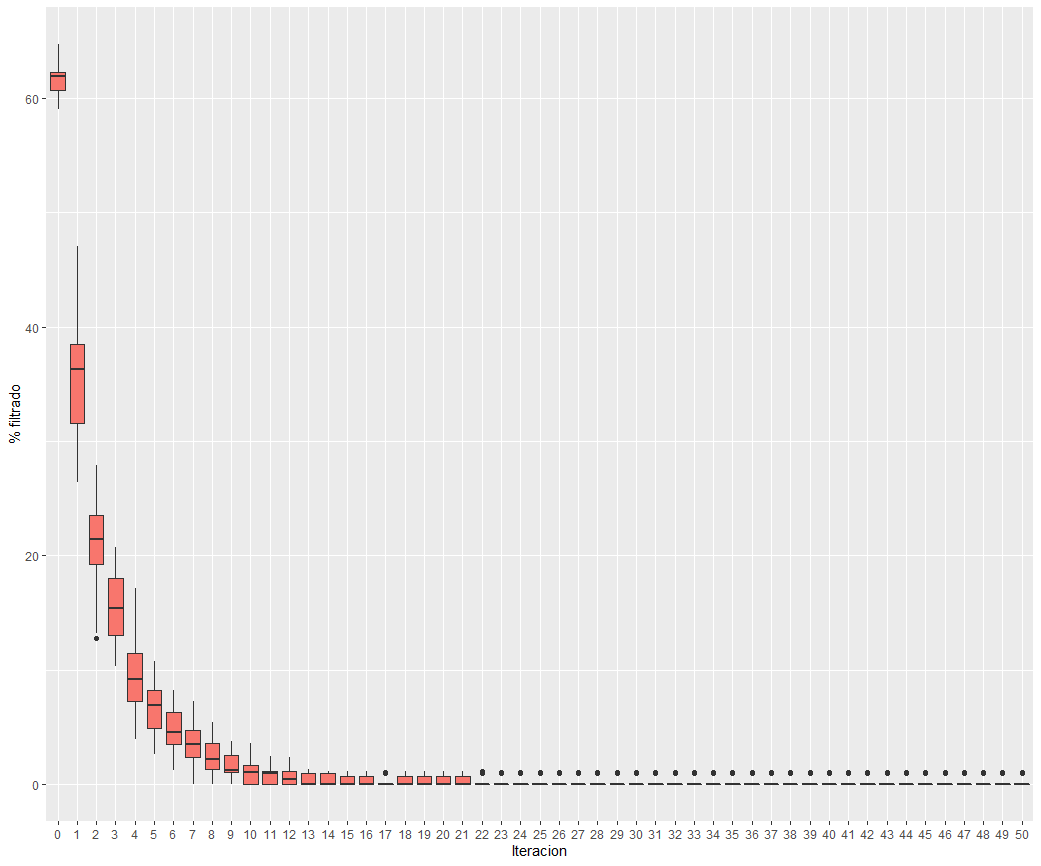
\includegraphics[width=87mm]{k100.png}}
\subfigure[k = 200]{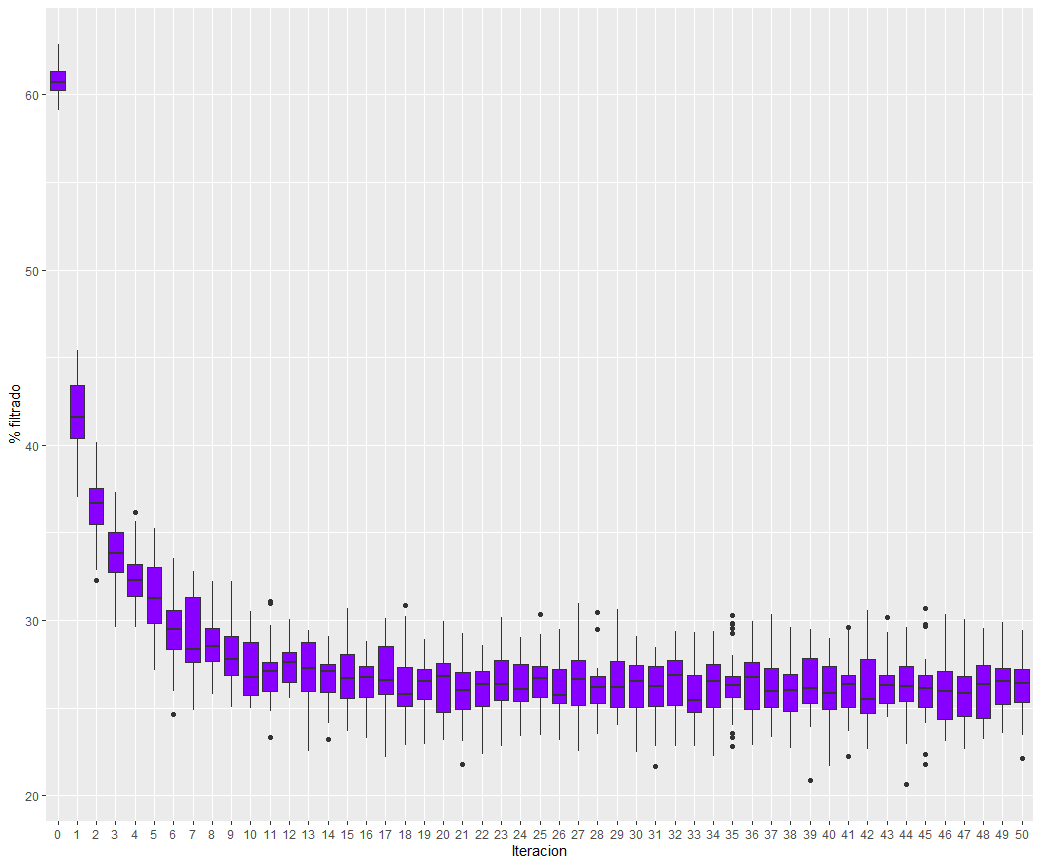
\includegraphics[width=87mm]{k200.png}}
\subfigure[k = 400]{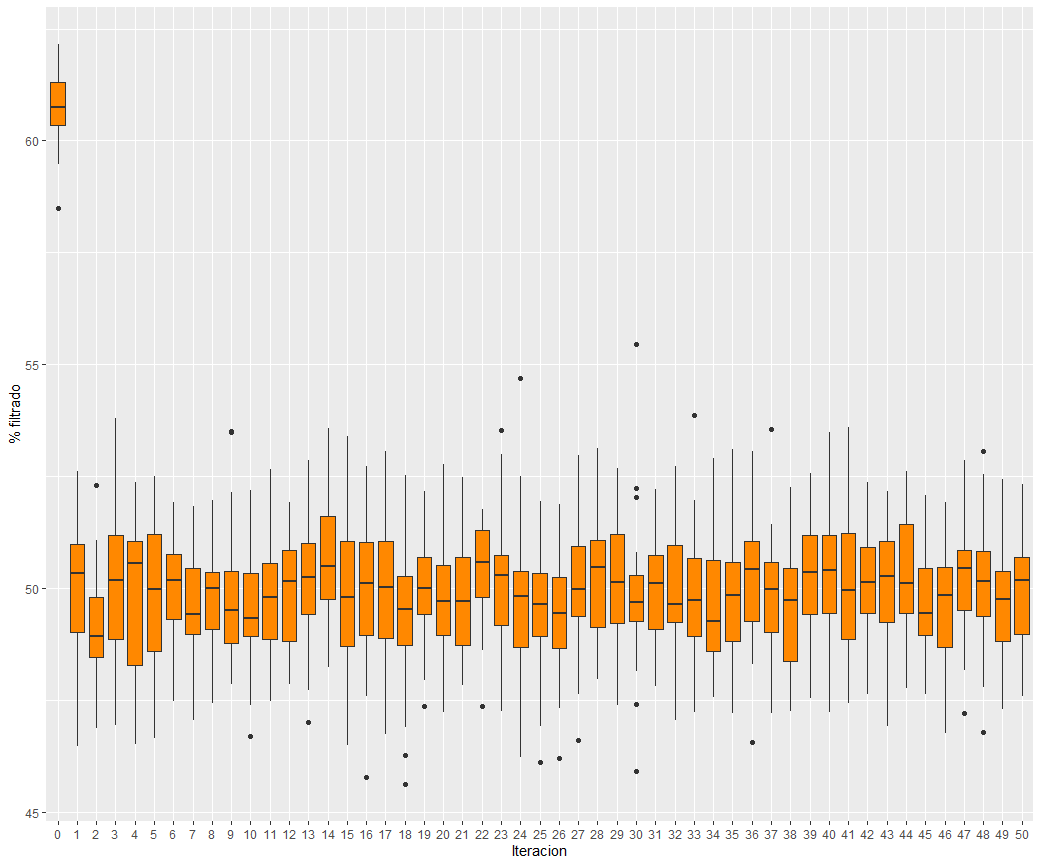
\includegraphics[width=87mm]{k400.png}}
\caption{Porcentaje de filtrado en cada iteración.} 
\label{f1}
\end{figure}

Los gifs \citep{2} de los histigramas de frecuencia relativa para cada paso simulando los fenómenos de rotura y agregación se encuentran en \href{https://github.com/nataliaperez0/Simulation/tree/main/Tarea8}{mi repositorio} en GitHub.
\smallskip

Para analizar si existe una relación entre la iteracion en que se realiza el filtrado y el porcentaje de filtrado que se obtiene se realizó una prueba estadística. Debido a los resultados obtenidos al revisar la normalidad de los datos, se eligió realizar la prueba estadística \texttt{Kruskal Wallis}.
\bigskip

En el cuadro \ref{Cuadro1} se  resumen los resultados de la revisión de los supuestos para poder aplicar la prueba y los resultados al aplicar la prueba estadística \texttt{Kruskal Wallis}. El supuesto outliers se refiere a la cantidad de valores atípicos que existen en los grupos y la normalidad se obtuvo con la prueba de \texttt{Shapiro Wilk}. En los resultados del cuadro \ref{Cuadro1} se observa que para todos los valores de $k$ no existe normalidad en los datos, ya que el valor de $p$ es menor a $0.05$, además al aplicar la prueba estadística también se obtienen valores de $p$ menores a $0.05$.

\newpage

\begin{table}[ht]
\centering
\caption{Resultados de los supuestos y de la prueba estadística \texttt{Kruskal Wallis}.}
\smallskip

\begin{tabular}{ |p{1cm}|p{1.5cm}|p{2cm}|p{2.3cm}|p{2cm}|}
 \hline
 k & Outliers & Normalidad & Chi cuadrada & Valor de $p$ \\
 \hline
 100 & 244 &  $2.02\times 10^{-58}$ & 6824.4 & $2.2\times 10^{-16}$ \\
 \hline
 200 & 139 & $1.68\times 10^{-51}$ & 6330.6 & $2.2\times 10^{-16}$ \\
 \hline
 400 & 38 & $2.89\times 10^{-41}$ & 7035.8 & $2.2\times 10^{-16}$ \\
 \hline
\end{tabular}
\label{Cuadro1}
\end{table}

Hipótesis nula : Las medias son iguales en todos los grupos.
\smallskip

Hipótesis alternativa: Debido a que $p < 0.05$ se rechaza la hipótesis nula, es decir que si existen diferencias significativas entre las medias de los grupos. 
\smallskip

Se entiende entonces que la iteración en la que se realiza el filtrado si tiene un efecto significativo en el porcentaje de cúmulos que se logran filtrar.
\bigskip

A continuación se muestra el código utilizado para realizar la prueba estadística \texttt{Kruskal Wallis}:

\lstset{style=mystyle}
\begin{lstlisting}[language=R, caption= Código para la prueba estadística \texttt{Kruskal Wallis}.]
library(tidyverse)
library(ggpubr)
library(car)
library(rstatix)
library(rapportools)
library(readr)
library(gridExtra)

#PRUEBA ESTADISTICA...
#Estadisticas descriptivas
#k = 100
dfs$`100` %>%
  group_by(k) %>%
  get_summary_stats(filtrado, type = "mean_sd")
#k = 200
dfs$`200` %>%
  group_by(k) %>%
  get_summary_stats(filtrado, type = "mean_sd")
#k = 400
dfs$`400` %>%
  group_by(k) %>%
  get_summary_stats(filtrado, type = "mean_sd")
#SUPUESTOS PARA ANOVA
#1:Outliers
#k = 100
dfs$`100` %>%
  group_by(k) %>%
  identify_outliers(filtrado)
#k = 200
dfs$`200` %>%
  group_by(k) %>%
  identify_outliers(filtrado)
#k = 400
dfs$`400` %>%
  group_by(k) %>%
  identify_outliers(filtrado)
#2:Normalidad por Shapiro
#k = 100
dfs$`100` %>%
  group_by(k) %>%
  shapiro_test(filtrado)
#k = 200
dfs$`200` %>%
  group_by(k) %>%
  shapiro_test(filtrado)
#k = 400
dfs$`400` %>%
  group_by(k) %>%
  shapiro_test(filtrado)
#3:Homogeneidad de varianza con prueba Levene
#k = 100
dfs$`100` %>%
  levene_test(filtrado$k)
#k = 200
dfs$`200` %>%
  levene_test(filtrado~k)
#k = 400
dfs$`400` %>%
  levene_test(filtrado~k)
#PRUEBA ESTADISTICA KRUSKAL WALLIS
#k = 100
dfs$`100` %>%
kruskal.test(filtrado ~ k)
#k = 200
dfs$`200` %>%
  kruskal.test(filtrado ~ k)
#k = 400
dfs$`400` %>%
  kruskal.test(filtrado ~ k)
#PRUEBA WILCOXON
pairwise.wilcox.test((dfs$`100`)$filtrado, (dfs$`100`)$Iteracion)
pairwise.wilcox.test((dfs$`200`)$filtrado, (dfs$`200`)$Iteracion)
pairwise.wilcox.test((dfs$`400`)$filtrado, (dfs$`200`)$Iteracion)
\end{lstlisting}

\section{Reto 1}
Como el primer reto, determina si existe algún intervalo de iteraciones en el que el filtrado alcance un óptimo. Realiza réplicas para determinar si el momento en el cual se alcanza el máximo tiene un comportamiento sistemático. Incluye visualizaciones para justificar las conclusiones.
\bigskip

En la figura \ref{f1} de la tarea base podemos notar que la mejor iteración para obtener el máximo porcentaje filtrado de cúmulos es la iteración $0$. En el cuadro \ref{Cuadro2} se muestra la iteración ideal para cada valor de $k$, el promedio de filtración que se obtiene y el promedio de tamaño crítico $c$ en cada valor de $k$.

\begin{table}[ht]
\centering
\caption{Iteración ideal para filtrar.}
\smallskip

\begin{tabular}{ |p{1cm}|p{1.5cm}|p{3.8cm}|p{2cm}|}
 \hline
 k & Iteración & Filtración promedio (\%) & $c$ promedio \\
 \hline
 100 & 0 &  $61.6$ & $966.5$ \\
 \hline
 200 & 0 & $60.9$ & $499$\\
 \hline
 400 & 0 & $60.2$ & $249$\\
 \hline
\end{tabular}
\label{Cuadro2}
\end{table}
\bigskip

En la figura \ref{f2} se muestra la iteración ideal para filtrar y obtener el mayor porcentaje de cúmulos filtrados en cada una de las $30$ réplicas para cada valor de $k$. Podemos apreciar que tanto para $k = 100$, $k = 200$ y $k = 400$ el mejor momento para filtrar es antes de comenzar las iteraciones debido a que existe un mayor porcentaje de cúmulos con un tamaño $c$ mayor o igual a la mediana de los cúmulos iniciales.
\bigskip

En \href{https://github.com/nataliaperez0/Simulation/tree/main/Tarea8}{mi repositorio}  de GitHub se encuentra el código realizado para este reto al cual solo se le agreron las instrucciones para realizar las gráficas de la figura \ref{f2} y para obtener los valores promedios de $filtración$ y $c$ mostrados en el cuadro \ref{Cuadro2}.

\begin{figure}[h!]
\centering
\subfigure[k = 100]{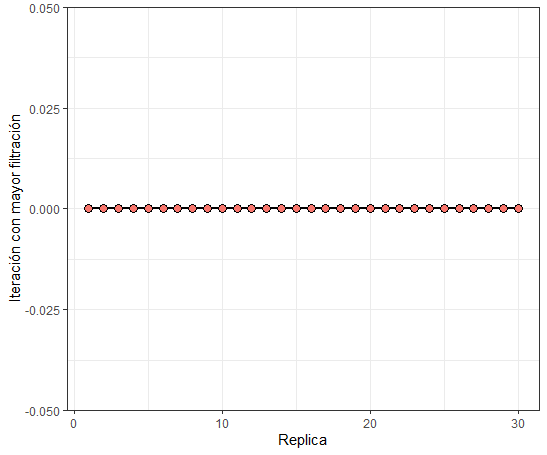
\includegraphics[width=87mm]{r1k100.png}}
\subfigure[k = 200]{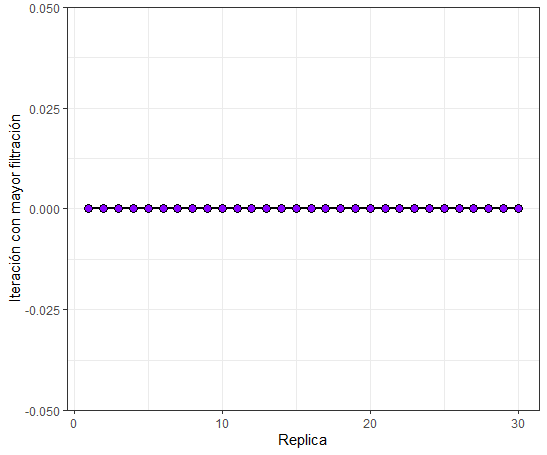
\includegraphics[width=87mm]{r1k200.png}}
\subfigure[k = 400]{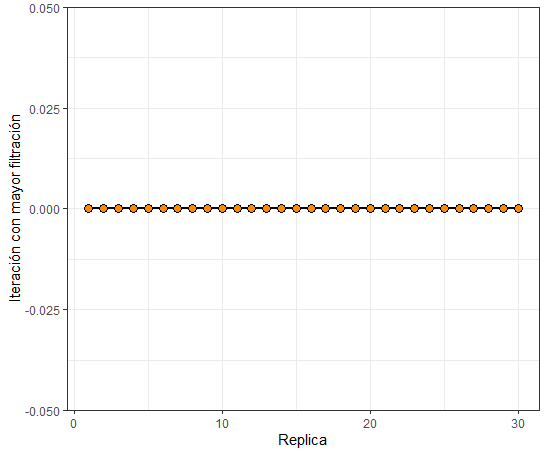
\includegraphics[width=87mm]{r1k400.png}}
\caption{Iteración con mayor porcentaje de filtración en cada réplica para cada valor $k$.} 
\label{f2}
\end{figure}

\newpage
\section{Reto 2}
Como un segundo reto, determina cómo los resultados de la tarea y del primer reto dependen del valor de $c$. ¿Qué cambia y cómo si $c$ ya no se asigna como la mediana inicial sino como un valor menor o mayor?.
\bigskip

Para este reto se utilizaron los siguientes valores de $c$ : $300, 600, 1200$ y $1800$, el valor de $c$ representa el tamaño crítico de los cúmulos por lo que también se podría denominar $filtro$ ya que en el código se establece que se deben filtrar los tamaños de cúmulos mayores o iguales a $c$. Al código objetivo de la tarea base se le agregó un ciclo \texttt{for} para variar el tamaño crítico de los cúmulos $c$ en los valores previamente mencionados y se realizaron diagramas caja-bigote para cada valor de $c$ con su respectivo valor $k$. En las figuras \ref{f3}, \ref{f4} y \ref{f5} se muestran los resultados obtenidos y en los cuadros \ref{Cuadro3}, \ref{Cuadro4} y \ref{Cuadro5} se indica la iteración ideal para cada tamaño crítico así como el promedio de filtración que se consigue en la respectiva iteración.

\newpage

\begin{figure}[h!]
\centering
\subfigure[k = 100 y c = 300]{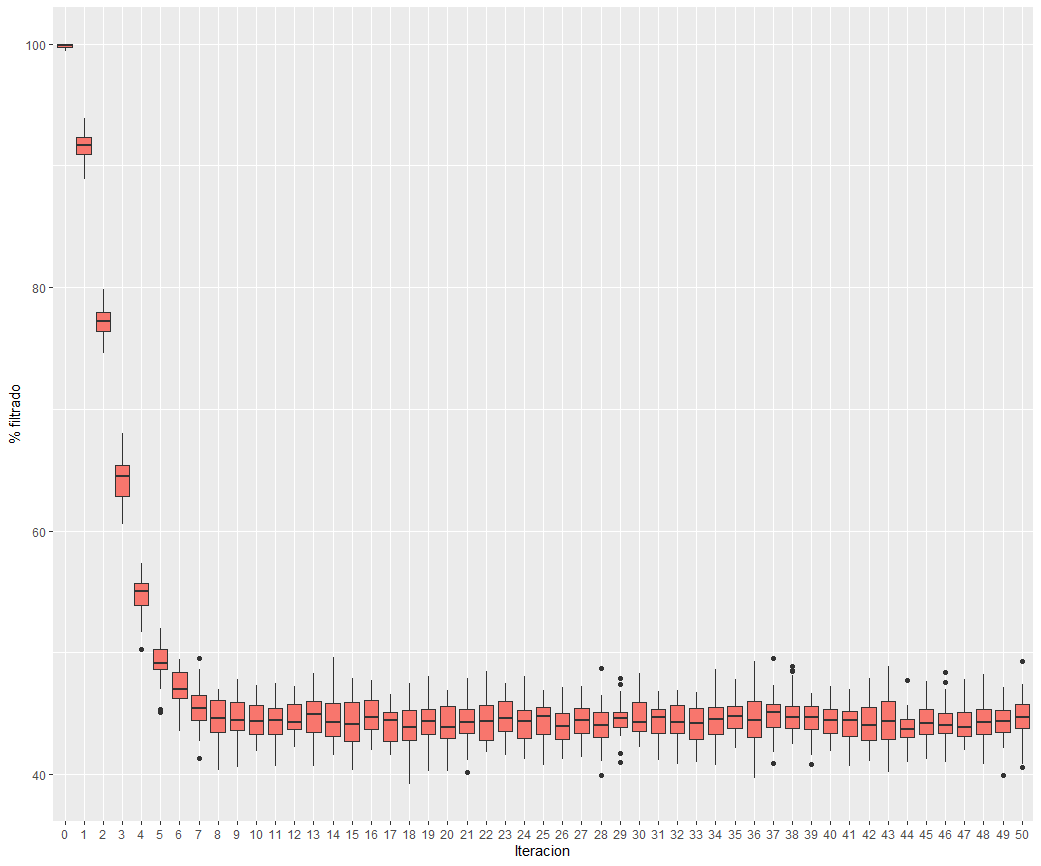
\includegraphics[width=87mm]{k100c300.png}}
\subfigure[k = 100 y c = 600]{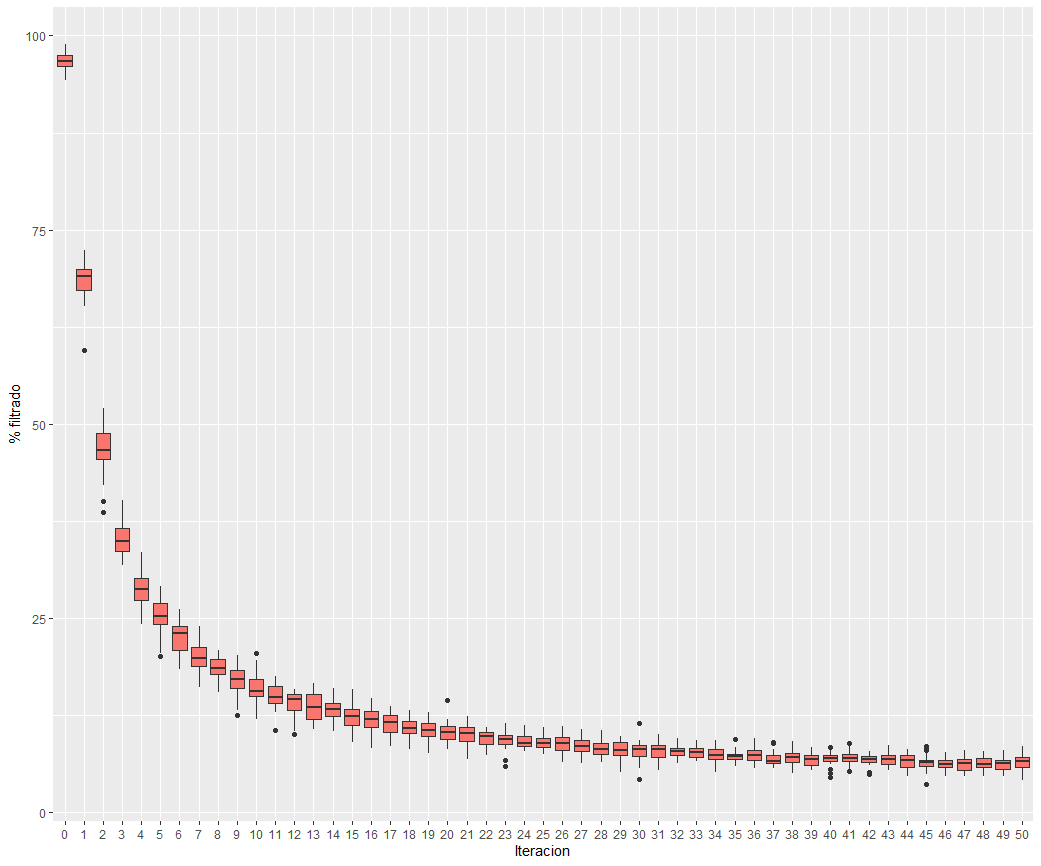
\includegraphics[width=87mm]{k100c600.png}}
\subfigure[k = 100 y c = 1200]{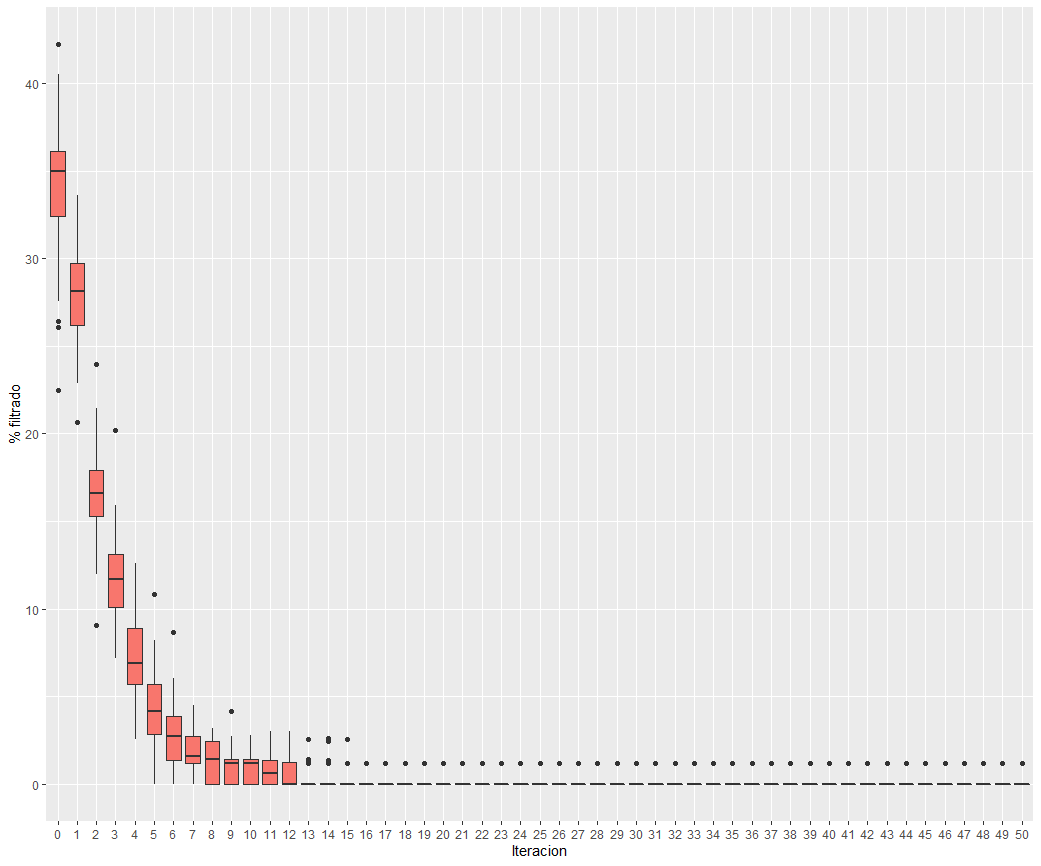
\includegraphics[width=87mm]{k100c1200.png}}
\subfigure[k = 100 y c = 1800]{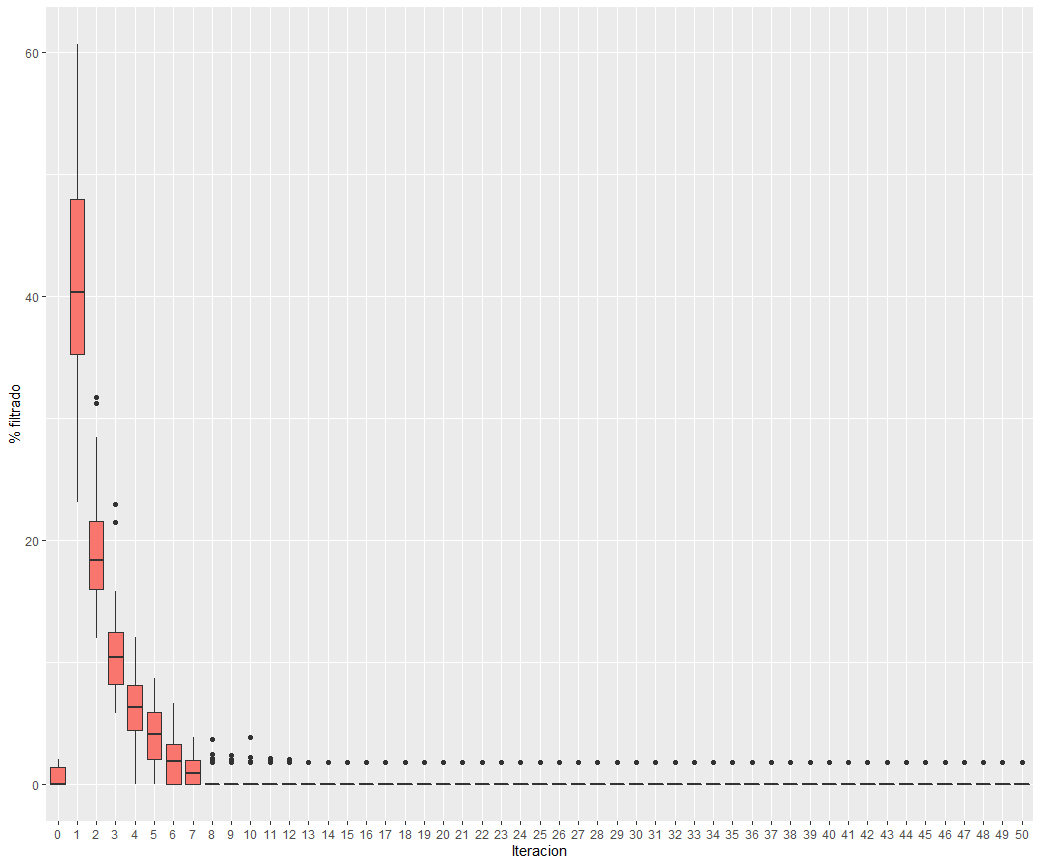
\includegraphics[width=87mm]{k100c1800.png}}
\caption{Porcentaje filtrado en cada iteración para cada tamaño crítico con $k = 100$.} 
\label{f3}
\end{figure}

\begin{table}[h!]
\centering
\caption{Iteración ideal para filtrar.}
\smallskip

\begin{tabular}{ |p{1cm}|p{1.5cm}|p{2cm}|p{3.8cm}|}
 \hline
 k & $c$ & Iteración & Filtración promedio (\%) \\
 \hline
 100 & 300 &  $0$ & $99.9$ \\
 \hline
 100 & 600 & $0$ & $96.6$\\
 \hline
 100 & 1200 & $0$ & $33.9$\\
 \hline
 100 & 1800 & $1$ & $41.9$\\
 \hline
\end{tabular}
\label{Cuadro3}
\end{table}

\newpage

\begin{figure}[h!]
\centering
\subfigure[k = 200 y c = 300]{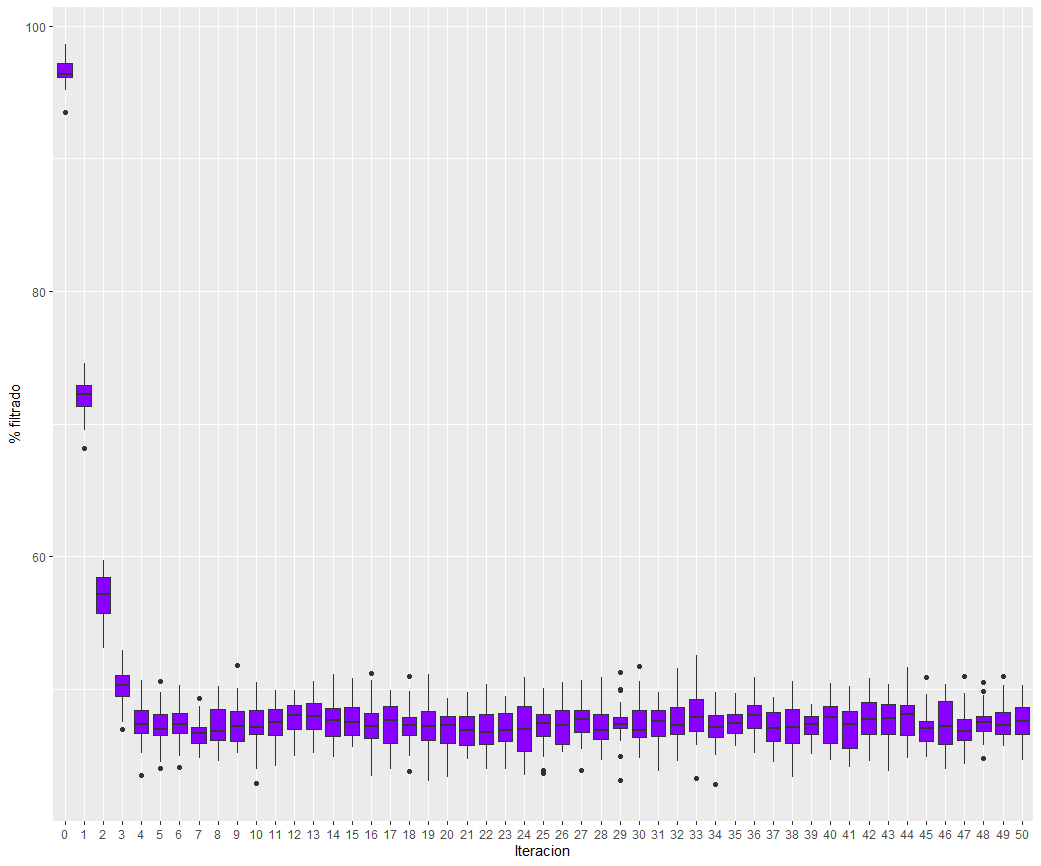
\includegraphics[width=87mm]{k200c300.png}}
\subfigure[k = 200 y c = 600]{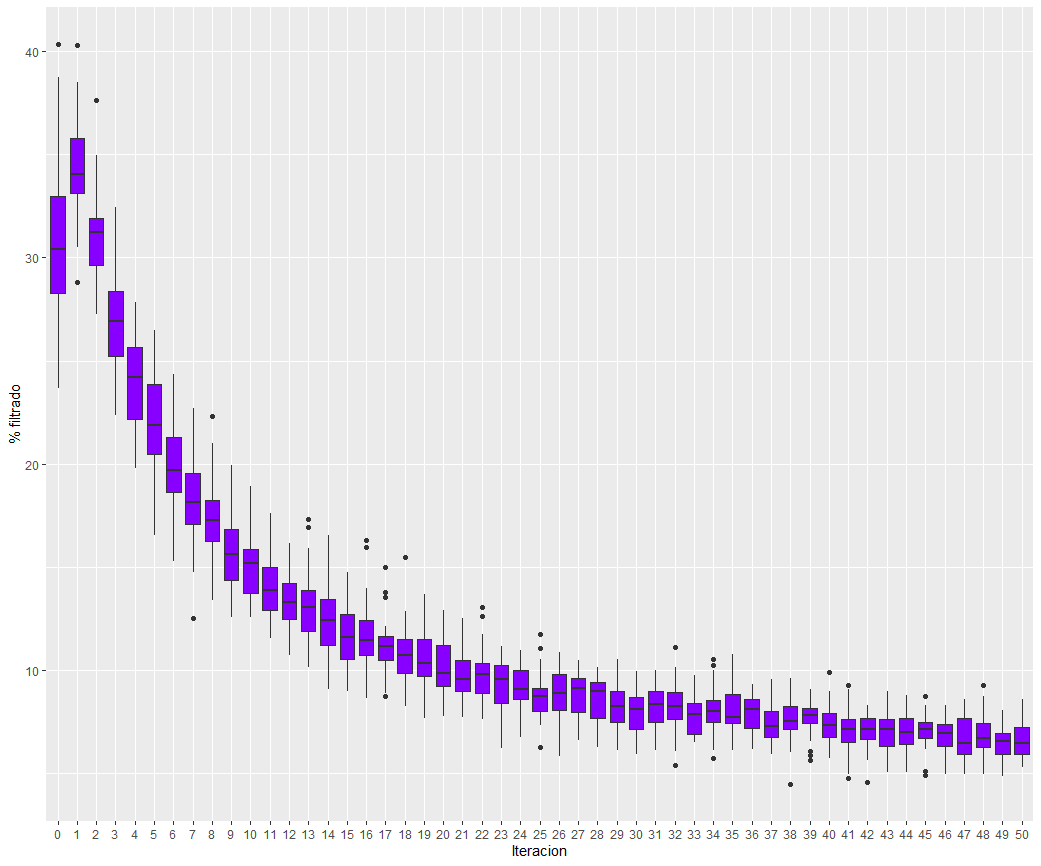
\includegraphics[width=87mm]{k200c600.png}}
\subfigure[k = 200 y c = 1200]{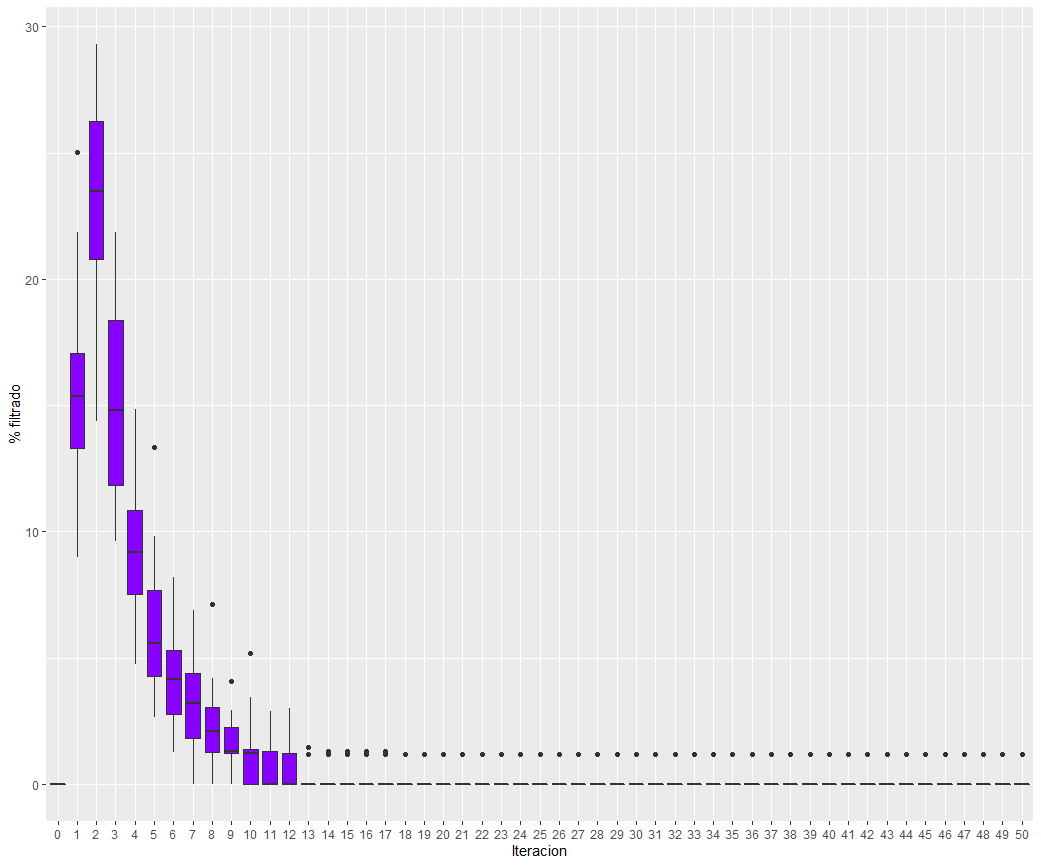
\includegraphics[width=87mm]{k200c1200.png}}
\subfigure[k = 200 y c = 1800]{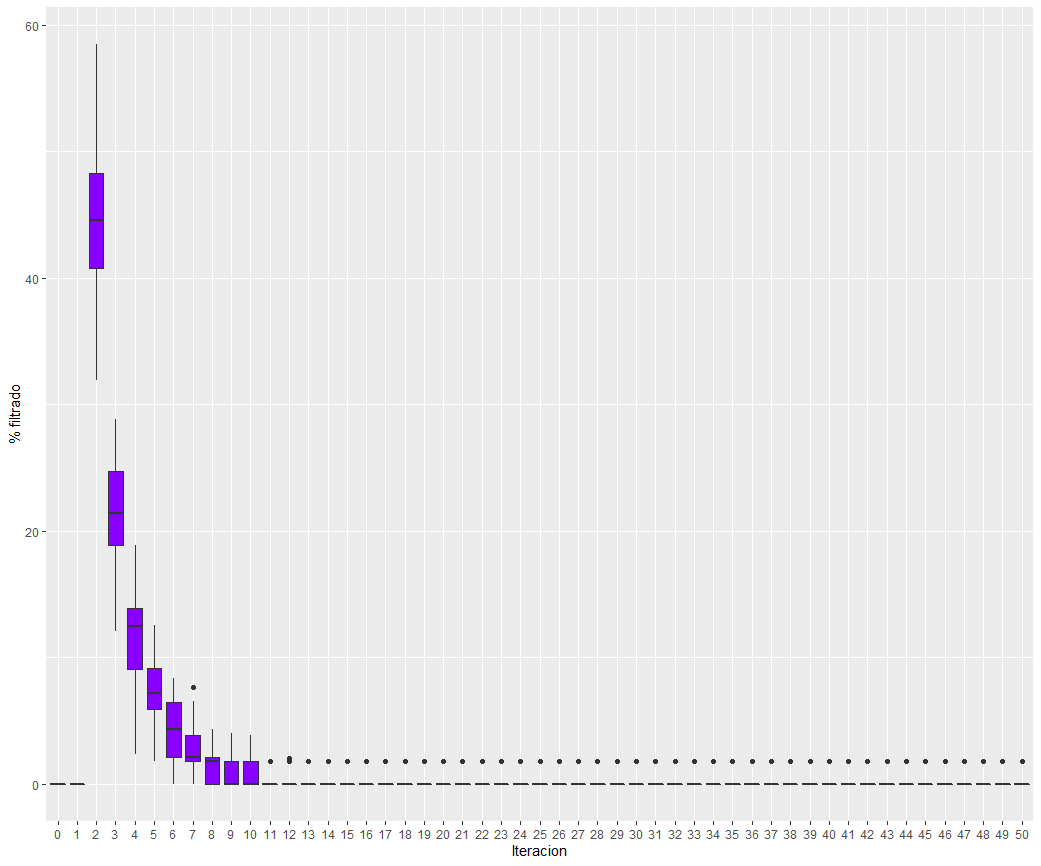
\includegraphics[width=87mm]{k200c1800.png}}
\caption{Porcentaje filtrado en cada iteración para cada tamaño crítico con $k = 200$.} 
\label{f4}
\end{figure}

\begin{table}[h!]
\centering
\caption{Iteración ideal para filtrar.}
\smallskip

\begin{tabular}{ |p{1cm}|p{1.5cm}|p{2cm}|p{3.8cm}|}
 \hline
 k & $c$ & Iteración & Filtración promedio (\%) \\
 \hline
 200 & 300 &  $0$ & $96.5$ \\
 \hline
 200 & 600 & $1$ & $34.4$\\
 \hline
 200 & 1200 & $2$ & $23.2$\\
 \hline
 200 & 1800 & $2$ & $44.4$\\
 \hline
\end{tabular}
\label{Cuadro4}
\end{table}

\newpage

\begin{figure}[h!]
\centering
\subfigure[k = 400 y c = 300]{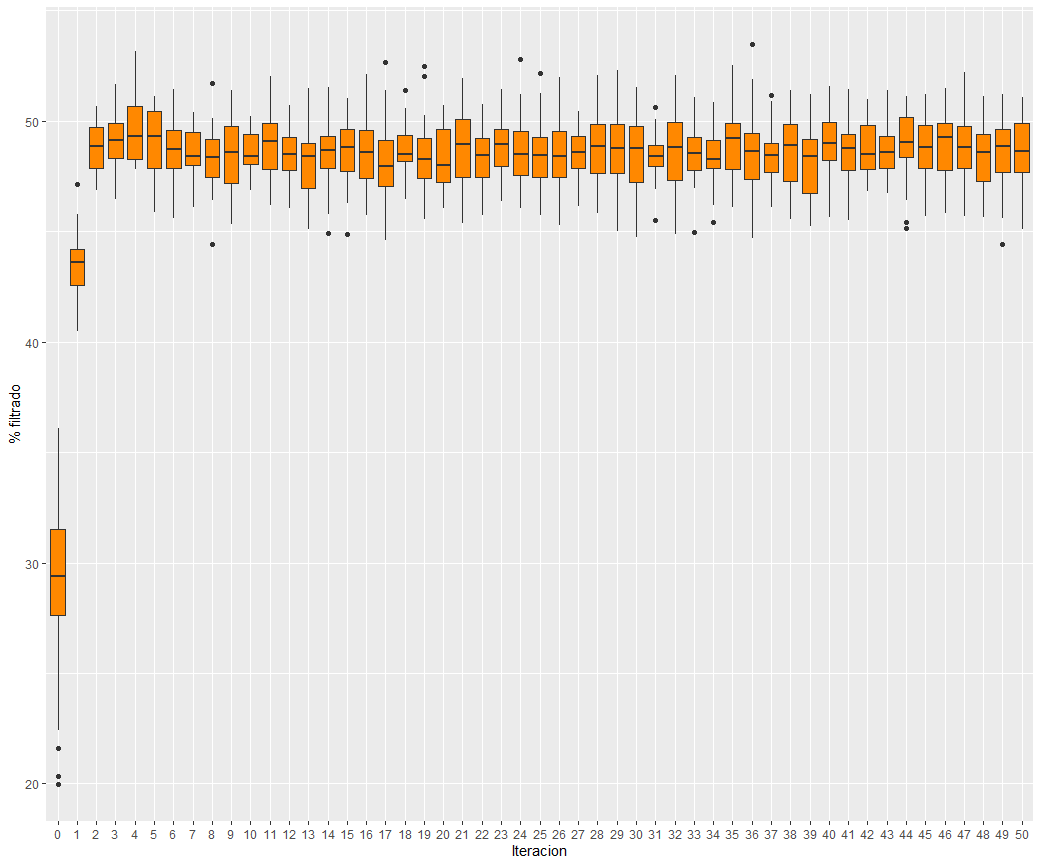
\includegraphics[width=87mm]{k400c300.png}}
\subfigure[k = 400 y c = 600]{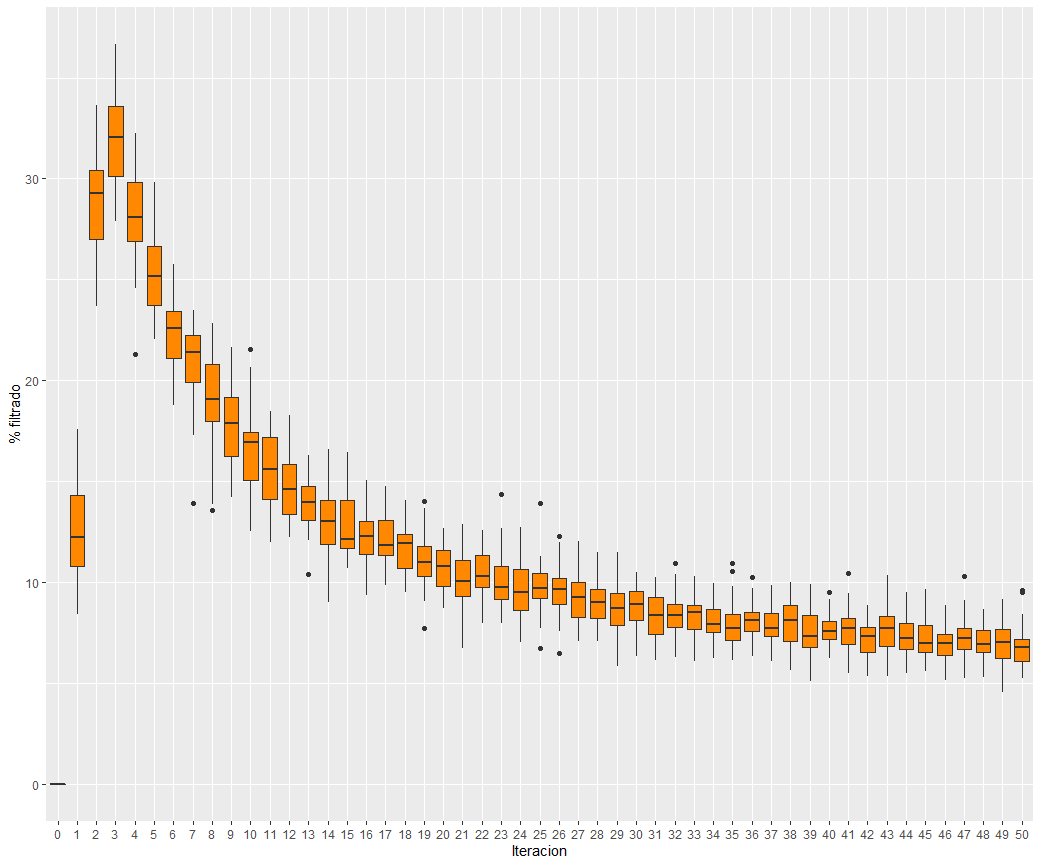
\includegraphics[width=87mm]{k400c600.png}}
\subfigure[k = 400 y c = 1200]{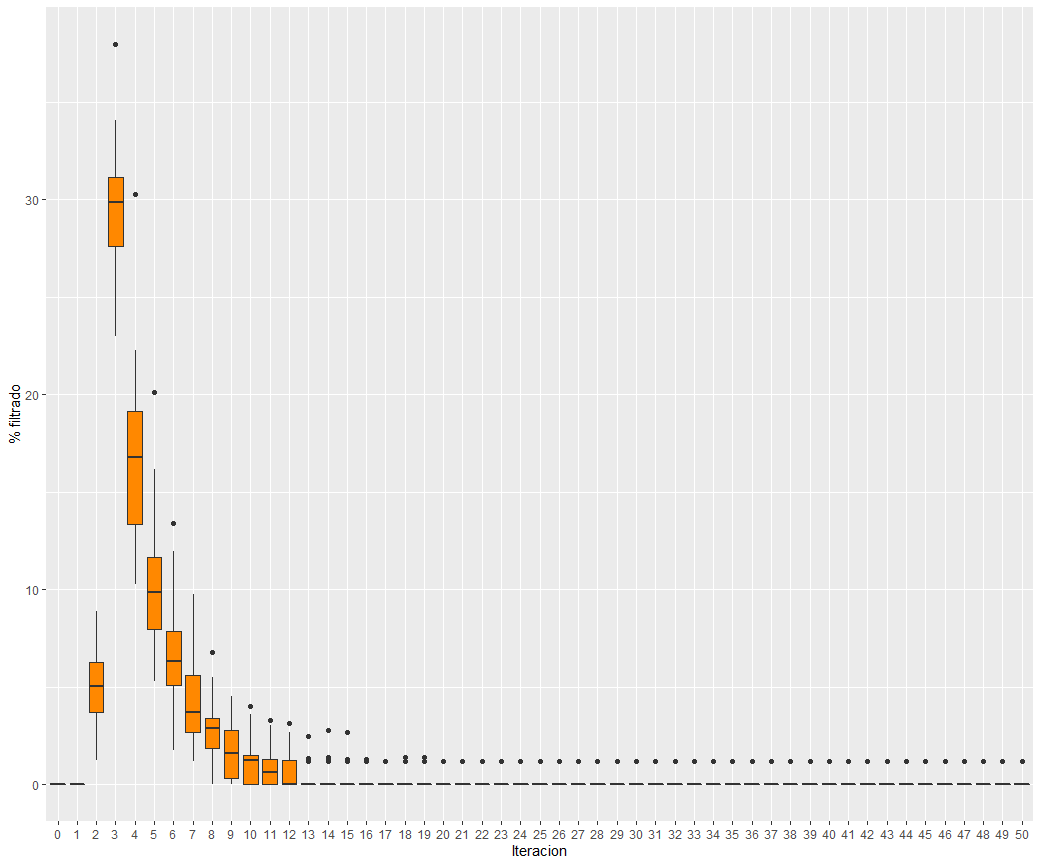
\includegraphics[width=87mm]{k400c1200.png}}
\subfigure[k = 400 y c = 1800]{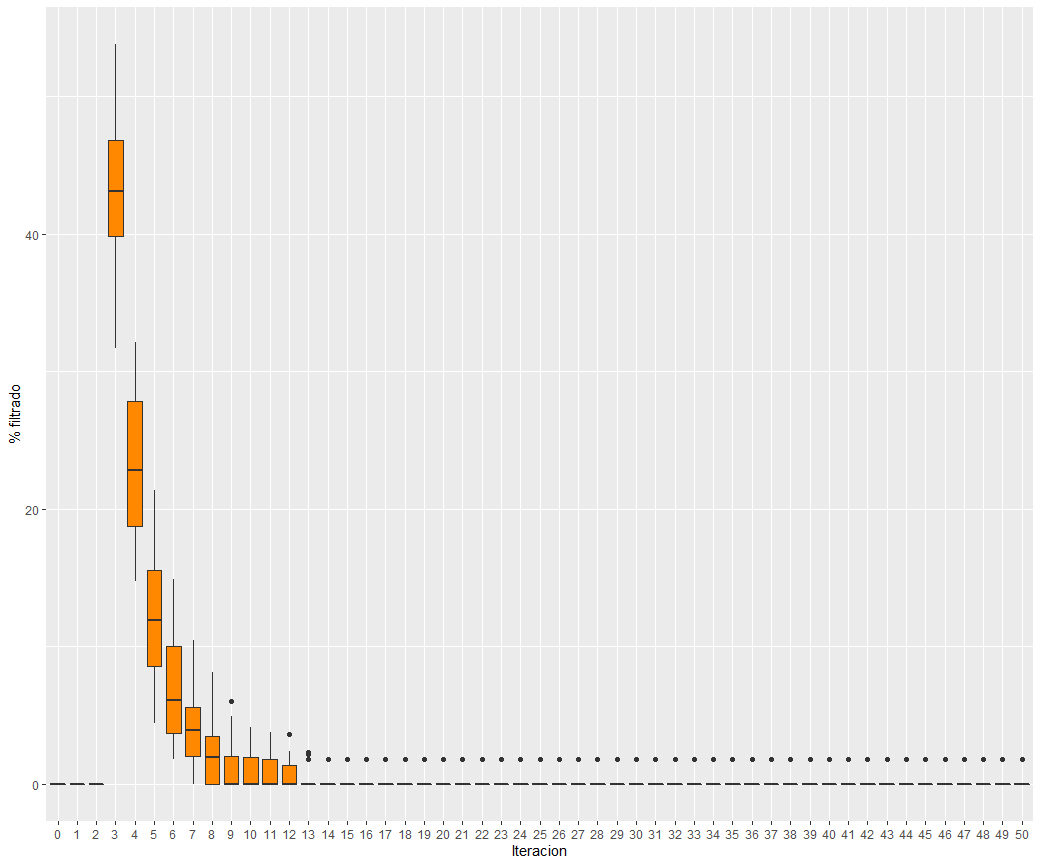
\includegraphics[width=87mm]{k400c1800.png}}
\caption{Porcentaje filtrado en cada iteración para cada tamaño crítico con $k = 400$.} 
\label{f5}
\end{figure}

\begin{table}[h!]
\centering
\caption{Iteración ideal para filtrar.}
\smallskip

\begin{tabular}{ |p{1cm}|p{1.5cm}|p{2cm}|p{3.8cm}|}
 \hline
 k & $c$ & Iteración & Filtración promedio (\%) \\
 \hline
 400 & 300 & $4$ & $49.6$ \\
 \hline
 400 & 600 & $3$ & $31.9$\\
 \hline
 400 & 1200 & $3$ & $29.6$\\
 \hline
 400 & 1800 & $2$ & $43.1$\\
 \hline
\end{tabular}
\label{Cuadro5}
\end{table}

A continuación se muestra el código generado para el reto $2$:

\definecolor{verde}{rgb}{0,0.56,0.22}
\definecolor{codegray}{rgb}{0.5,0.5,0.5}
\definecolor{codegreen}{rgb}{0,0.56,0.22}
\definecolor{backcolour}{rgb}{0.95,0.95,0.92}
\definecolor{azul}{rgb}{0,0,1}

\lstdefinestyle{mystyle}{
    backgroundcolor=\color{backcolour},   
    commentstyle=\color{verde},
    keywordstyle=\color{azul},
    numberstyle=\tiny\color{codegray},
    stringstyle=\color{codegreen},
    basicstyle=\ttfamily\footnotesize,
    breakatwhitespace=false,         
    breaklines=true,                 
    captionpos=b,                    
    keepspaces=true,                 
    numbers=left,                    
    numbersep=5pt,                  
    showspaces=false,                
    showstringspaces=false,
    showtabs=false,                  
    tabsize=2
}

\lstset{style=mystyle}
\begin{lstlisting}[language=R, caption= Código para graficar el porcentaje de filtrado en cada iteración.]
library(testit) # para pruebas, recuerda instalar antes de usar
tamas <- c(100, 200, 400)
n <- 100000
df = data.frame()
se = c(300, 600, 1200, 1800)

for (k in tamas){
  for (c in se){
    for (replica in 1:30){
      originales <- rnorm(k)
      cumulos <- originales - min(originales) + 1
      cumulos <- round(n * cumulos / sum(cumulos))
      assert(min(cumulos) > 0)
      diferencia <- n - sum(cumulos)
      if (diferencia > 0) {
        for (i in 1:diferencia) {
          p <- sample(1:k, 1)
          cumulos[p] <- cumulos[p] + 1
        }
      } else if (diferencia < 0) {
        for (i in 1:-diferencia) {
          p <- sample(1:k, 1)
          if (cumulos[p] > 1) {
            cumulos[p] <- cumulos[p] - 1
          }
        }
      }
      
      assert(length(cumulos[cumulos == 0]) == 0) # que no haya vacios
      assert(sum(cumulos) == n)
      
      d <- sd(cumulos) / 4 # factor arbitrario para suavizar la curva
      
      primero <- as.data.frame(table(cumulos))
      names(primero) <- c("tam", "num")
      primero$tam <- as.numeric(levels(primero$tam))[primero$tam]
      assert(sum(primero$num * primero$tam) == n)
      
      filtrados1 = primero[primero$tam >= c,]
      filtrados1$cont = filtrados1$tam * filtrados1$num
      f1 = sum(filtrados1$cont) # particulas removidas
      porcentaje1 = 100 * f1/n # porcentaje exitosamente filtrado
      paso1 = 0
      resultado1 = c(k, replica, paso1, porcentaje1, c)
      df = rbind(df, resultado1)
      names(df) = c("k", "Replica", "Iteracion", "filtrado", "c")
      assert(sum(abs(cumulos)) == n)
      
      rotura <- function(x) {
        return (1 / (1 + exp((c - x) / d)))
      }
      union <- function(x) {
        return (exp(-x / c))
      }
      romperse <- function(tam, cuantos) {
        romper <- round(rotura(tam) * cuantos) # independientes
        resultado <- rep(tam, cuantos - romper) # los demas
        if (romper > 0) {
          for (cumulo in 1:romper) { # agregar las rotas
            t <- 1
            if (tam > 2) { # sample no jala con un solo valor
              t <- sample(1:(tam-1), 1)
            }
            resultado <- c(resultado, t, tam - t)
          }
        }
        assert(sum(resultado) == tam * cuantos) # no hubo perdidas
        return(resultado)
      }
      unirse <- function(tam, cuantos) {
        unir <- round(union(tam) * cuantos) # independientes
        if (unir > 0) {
          division <- c(rep(-tam, unir), rep(tam, cuantos - unir))
          assert(sum(abs(division)) == tam * cuantos)
          return(division)
        } else {
          return(rep(tam, cuantos))
        }
      }
      freq <- as.data.frame(table(cumulos))
      names(freq) <- c("tam", "num")
      freq$tam <- as.numeric(levels(freq$tam))[freq$tam]
      duracion <- 50
      digitos <- floor(log(duracion, 10)) + 1
      for (paso in 1:duracion) {
        assert(sum(cumulos) == n)
        cumulos <- integer()
        for (i in 1:dim(freq)[1]) { # fase de rotura
          urna <- freq[i,]
          if (urna$tam > 1) { # no tiene caso romper si no se puede
            cumulos <- c(cumulos, romperse(urna$tam, urna$num))
          } else {
            cumulos <- c(cumulos, rep(1, urna$num))
          }
        }
        assert(sum(cumulos) == n)
        assert(length(cumulos[cumulos == 0]) == 0) # que no haya vacios
        freq <- as.data.frame(table(cumulos)) # actualizar urnas
        names(freq) <- c("tam", "num")
        freq$tam <- as.numeric(levels(freq$tam))[freq$tam]
        assert(sum(freq$num * freq$tam) == n)
        cumulos <- integer()
        for (i in 1:dim(freq)[1]) { # fase de union
          urna <- freq[i,]
          cumulos <- c(cumulos, unirse(urna$tam, urna$num))
        }
        assert(sum(abs(cumulos)) == n)
        assert(length(cumulos[cumulos == 0]) == 0) # que no haya vacios
        juntarse <- -cumulos[cumulos < 0]
        cumulos <- cumulos[cumulos > 0]
        assert(sum(cumulos) + sum(juntarse) == n)
        nt <- length(juntarse)
        if (nt > 0) {
          if (nt > 1) {
            juntarse <- sample(juntarse)
            for (i in 1:floor(nt / 2) ) {
              cumulos <- c(cumulos, juntarse[2*i-1] + juntarse[2*i])
            }
          }
          if (nt %% 2 == 1) {
            cumulos <- c(cumulos, juntarse[nt])
          }
        }
        assert(sum(cumulos) == n)
        freq <- as.data.frame(table(cumulos))
        names(freq) <- c("tam", "num")
        freq$tam <- as.numeric(levels(freq$tam))[freq$tam]
        assert(sum(freq$num * freq$tam) == n)
        tl <- paste(paso, "", sep="")
        while (nchar(tl) < digitos) {
          tl <- paste("0", tl, sep="")
        }

        freq
        filtrados = freq[freq$tam >= c,]
        filtrados$cont = filtrados$tam * filtrados$num
        f = sum(filtrados$cont) # particulas removidas
        porcentaje = 100 * f/n # porcentaje exitosamente filtrado
        resultado = c(k, replica, paso, porcentaje, c)
        df = rbind(df, resultado)
        
        assert(sum(abs(cumulos)) == n)
      }  
    }
  } 
}


a1 = df[df$k == 100 & df$c == 300, ]
a2 = df[df$k == 100 & df$c == 600, ]
a3 = df[df$k == 100 & df$c == 1200, ]
a4 = df[df$k == 100 & df$c == 1800, ]

b1 = df[df$k == 200 & df$c == 300, ]
b2 = df[df$k == 200 & df$c == 600, ]
b3 = df[df$k == 200 & df$c == 1200, ]
b4 = df[df$k == 200 & df$c == 1800, ]

c1 = df[df$k == 400 & df$c == 300, ]
c2 = df[df$k == 400 & df$c == 600, ]
c3 = df[df$k == 400 & df$c == 1200, ]
c4 = df[df$k == 400 & df$c == 1800, ]

library(ggplot2)
a1$Iteracion = as.factor(a1$Iteracion)
ggplot(a1, aes(x= Iteracion, y= filtrado)) + 
  geom_boxplot(fill = "#F8766D")+
  labs(x = "Iteracion", y = "% filtrado", title = 'k = 100 y c = 300')

a2$Iteracion = as.factor(a2$Iteracion)
ggplot(a2, aes(x= Iteracion, y= filtrado)) + 
  geom_boxplot(fill = "#F8766D")+
  labs(x = "Iteracion", y = "% filtrado", title = 'k = 100 y c = 600')

a3$Iteracion = as.factor(a3$Iteracion)
ggplot(a3, aes(x= Iteracion, y= filtrado)) + 
  geom_boxplot(fill = "#F8766D")+
  labs(x = "Iteracion", y = "% filtrado", title = 'k = 100 y c = 1200')

a4$Iteracion = as.factor(a4$Iteracion)
ggplot(a4, aes(x= Iteracion, y= filtrado)) + 
  geom_boxplot(fill = "#F8766D")+
  labs(x = "Iteracion", y = "% filtrado", title = 'k = 100 y c = 1800')

b1$Iteracion = as.factor(b1$Iteracion)
ggplot(b1, aes(x= Iteracion, y= filtrado)) + 
  geom_boxplot(fill = "#8800FF")+
  labs(x = "Iteracion", y = "% filtrado", title = 'k = 200 y c = 300')

b2$Iteracion = as.factor(b2$Iteracion)
ggplot(b2, aes(x= Iteracion, y= filtrado)) + 
  geom_boxplot(fill = "#8800FF")+
  labs(x = "Iteracion", y = "% filtrado", title = 'k = 200 y c = 600')

b3$Iteracion = as.factor(b3$Iteracion)
ggplot(b3, aes(x= Iteracion, y= filtrado)) + 
  geom_boxplot(fill = "#8800FF")+
  labs(x = "Iteracion", y = "% filtrado", title = 'k = 200 y c = 1200')

b4$Iteracion = as.factor(b4$Iteracion)
ggplot(b4, aes(x= Iteracion, y= filtrado)) + 
  geom_boxplot(fill = "#8800FF")+
  labs(x = "Iteracion", y = "% filtrado", title = 'k = 200 y c = 1800')

c1$Iteracion = as.factor(c1$Iteracion)
ggplot(c1, aes(x= Iteracion, y= filtrado)) + 
  geom_boxplot(fill = "#FF8800")+
  labs(x = "Iteracion", y = "% filtrado", title = 'k = 400 y c = 300')

c2$Iteracion = as.factor(c2$Iteracion)
ggplot(c2, aes(x= Iteracion, y= filtrado)) + 
  geom_boxplot(fill = "#FF8800")+
  labs(x = "Iteracion", y = "% filtrado", title = 'k = 400 y c = 600')

c3$Iteracion = as.factor(c3$Iteracion)
ggplot(c3, aes(x= Iteracion, y= filtrado)) + 
  geom_boxplot(fill = "#FF8800")+
  labs(x = "Iteracion", y = "% filtrado", title = 'k = 400 y c = 1200')

c4$Iteracion = as.factor(c4$Iteracion)
ggplot(c4, aes(x= Iteracion, y= filtrado)) + 
  geom_boxplot(fill = "#FF8800")+
  labs(x = "Iteracion", y = "% filtrado")

a1[a1$Iteracion == 0,] %>%
  get_summary_stats(filtrado, type = "mean_sd")

a2[a2$Iteracion == 0,] %>%
  get_summary_stats(filtrado, type = "mean_sd")

a3[a3$Iteracion == 0,] %>%
  get_summary_stats(filtrado, type = "mean_sd")

a4[a4$Iteracion == 1,] %>%
  get_summary_stats(filtrado, type = "mean_sd")

b1[b1$Iteracion == 0,] %>%
  get_summary_stats(filtrado, type = "mean_sd")

b2[b2$Iteracion == 1,] %>%
  get_summary_stats(filtrado, type = "mean_sd")

b3[b3$Iteracion == 2,] %>%
  get_summary_stats(filtrado, type = "mean_sd")

b4[b4$Iteracion == 2,] %>%
  get_summary_stats(filtrado, type = "mean_sd")

c1[c1$Iteracion == 0,] %>%
  get_summary_stats(filtrado, type = "mean_sd")

g1 =c1 %>%
  group_by(Iteracion) %>%
  get_summary_stats(filtrado, type = "mean_sd")

g1 %>%
  get_summary_stats(mean, type = "max")

c2[c2$Iteracion == 3,] %>%
  get_summary_stats(filtrado, type = "mean_sd")

c3[c3$Iteracion == 3,] %>%
  get_summary_stats(filtrado, type = "mean_sd")

c4[c4$Iteracion == 3,] %>%
  get_summary_stats(filtrado, type = "mean_sd")
\end{lstlisting}

\newpage
\section{Conclusi\'{o}n}
Con base en los diagramas caja-bigote y el resultado obtenido de la prueba estadística \texttt{Kruskal Wallis} para la tarea base, puedo concluir que la iteración en que se realiza el proceso de filtrado si afecta el porcentaje de cúmulos filtrados, y si el filtro que se utiliza es la mediana de los cúmulos el momento ideal para filtrar será antes de comenzar las iteraciones ya que existen más cúmulos mayores o iguales al tamaño del $filtro$. De igual manera si el tamaño del $filtro$ es menor que la mediana de los cúmulos también se tendrá como momento ideal para filtrar la iteración $0$, sin embargo si el tamaño del $filtro$ es mayor que la mediana de los cúmulos la iteración ideal para filtrar no será precisamente la $0$ pero si durante las primeras iteraciones.
\smallskip

En general ésta práctica fue mucho de mi agrado ya que no tuve grandes dificultades para realizarla y aprendí a manipular mejor los \texttt{data.frame} en \texttt{RStudio}.
\newpage

\bibliography{referencias}
\bibliographystyle{plainnat}

\end{document}